% !TeX encoding = UTF-8
\section{Gute Gründe für Traumap{\"a}dagogik – worüber gesprochen wird}

Traumapädagogik ist als Antwort auf die Überforderung der pädagogischen Praxis mit traumatisierten Kindern und Jugendlichen entstanden (vgl. Kühn 2014: 25). Dieser Überforderung will Traumapädagogik mit entsprechenden Haltungen und Konzepten begegnen. Vorliegendes Kapitel widmet sich der Frage, warum es der Traumapädagogik bedürfe. Im Folgenden werden Argumente, die in der Literatur zu finden sind und für die Traumapädagogik sprechen sollen, beschrieben. Das Kapitel fokussiert: die Häufigkeit der Belastungen der Kinder und Jugendlichen (3.1), deren besondere Bedarfe (3.2), den Beitrag der Traumapädagogik zur Entlastung der pädagogischen Praxis (3.3) sowie ihre Bedeutung für den pädagogischen Alltag (3.4).

\subsection{Es sind viele!}
Die hohen Zahlen der Kinder und Jugendlichen, die belastenden, traumatischen Erlebnissen ausgesetzten waren, soll die Bedeutung der Psychotraumatologie für deren (therapeutische) Unterstützung beweisen (vgl. Landolt \& Hensel 2008: 13). Daten, die die tatsächliche Anzahl traumatisierter Kinder und Jugendlicher in Deutschland verlässlich abbilden könnten, gibt es nicht (vgl. Bundesministerium für Familie, Senioren, Frauen und Jugend [BMFSFJ] 2009: 238). Häufig werden Studien und Zahlen zitiert, die die Anwesenheit psychisch belasteter Kindern und Jugendlicher in verschiedenen pädagogischen Institutionen beweisen sollen. Die berichteten Zahlen der potenziell oder tatsächlich Traumatisierten variieren zwischen 60 und 85\% bei den fremdplatzierten Kindern (vgl. Schmid 2013: 36 ff.). Als besonders belastet gelten laut diesen Ergebnissen Mädchen und Jungen, die in den stationären Einrichtungen der Jugendhilfe untergebracht sind und besonders häufig Vernachlässigung und Misshandlungsrisiken ausgesetzt waren (vgl. ebd.). Der Großteil der Kinder in Heimen weise Typ-II-Traumatisierungen auf und leide an einer komplexen posttraumatischen Belastungsstörung oder Traumaentwicklungsstörung (s. u., vgl. Schmid 2013: 37). Viele Kinder und Jugendlichen in der Jugendhilfe zeigten in der Diagnostik gleichzeitig mehrere psychische Erkrankungen, was deren besonderen Unterstützungsbedarf beweise (vgl. Schmid 2013: 38). Somit gelte für die Einrichtungen der station{\"a}ren Jugendhilfe, dass früh misshandelte, missbrauchte und vernachlässigte Kinder eher die Regel als Ausnahme seien (vgl. ebd.: 36). Aus diesen Erkenntnissen sowie aus der Tatsache, dass die KlientInnen der Jugendhilfe auch externe Einrichtungen wie z. B. Schulen besuchen, werden Bedarfe an den traumapädagogischen Konzepten auch für diese abgeleitet (vgl. Möhrlein \& Hoffart 2014: 91 ff.). Momentan ist ein Anstieg wissenschaftlicher Publikationen zum Thema der Lebenssituationen minderj{\"a}hriger Fl{\"u}chtlinge zu beobachten (vgl. Reinelt u. a. 2016: 232 f.). Das Interesse an der Thematik der psychischen Gesundheit gefl{\"u}chteter Kinder und Jugendlichen steigt. Besonders viel wird über das m{\"o}gliche Auftreten einer posttraumatischen Belastungsst{\"o}rung und ihre Behandlung publiziert (vgl. ebd.).

\subsection{Besondere Bedarfe traumatisierter Kinder und Jugendlicher}
Der spezifische pädagogische Bedarf der komplex traumatisierten Kinder und Jugendlichen ergibt sich laut Schmid (2013: 47) aus den Traumafolgen. Einmalige traumatische Ereignisse sind meist leichter zu erkennen und therapeutisch zu begleiten, als das bei den chronischen und wiederkehrenden Erfahrungen (z. B. Kindesmisshandlung) der Fall ist.  

Die systematische Auseinandersetzung mit kindlichen Reaktionen auf traumatische Ereignisse ist in der Kinderpsychotherapie noch recht jung (vgl. Landolt \& Hensel 2008: 13). Erst im Jahre 1988 wurde das Vorhandensein der posttraumatischen Belastungsstörung (PTBS) auch bei Kindern anerkannt (vgl. ebd.). Gleichzeitig ist die PTBS weder die typische noch die häufigste Traumafolgestörung bei Kindern und Jugendlichen (vgl. Hensel 2014: 27). Traumatische Erlebnisse in der Kindheit wirken sich auf die emotionale, kognitive und soziale Entwicklung der Kinder und Jugendlichen aus (vgl. Purtscher-Penz 2015: 95). Folgen einer lebensbedrohlichen Erfahrung, etwa eines Unfalls, sexuellen Missbrauchs, Verlusts einer nahen Bezugsperson etc., können psychische Erkrankungen, somatische Beschwerden, Lernprobleme sowie Störungen des Sozialverhaltens sein. Auch stressbezogene Alltagserfahrungen können zu traumareaktiven Folgeerkrankungen führen. Wiederholte Stressereignisse und chronisches Stresserleben verursachen eine komplexe Traumatisierung bei Kindern und Jugendlichen. Nur wenige dieser Kinder zeigen traumaspezifische Folgeerkrankungen im klinischen Sinne (vgl. ebd.). Da die vielfältigen und komplexen Folgen der frühkindlichen Traumatisierung in den bisherigen Diagnosen nicht berücksichtigt seien, wird eine Diagnose von entwicklungsbezogenen Traumafolgestörungen (vgl. Purtscher-Penz 2015: 97) bzw. Traumaentwicklungsstörungen (mehr dazu: Schmid u. a. 2010) diskutiert. Die Herausforderungen für die (sozial-)pädagogische Praxis, die sich laut Schmid (2013: 43) aus den Folgen komplexer Traumatisierungen ergeben, fasst die untenstehende Abbildung \ref{fig:folgen} zusammen.

Diese Herausforderungen lassen wiederum auf einen spezifischen pädagogischen Bedarf der betroffenen Kinder und Jugendlichen sowie entsprechende Interventionen schließen (vgl. Schmid 2013: 47; siehe Abbildung \ref{fig:ansatzpunkte}: \pageref{fig:ansatzpunkte}). Da diese Kinder häufige Beziehungsabbrüche und Wechsel von Bezugspersonen erlebt haben, brauchen sie Sicherheit und Verlässlichkeit im Alltag, was die Verlässlichkeit von Bezugspersonen, getroffenen Vereinbarungen und Absprachen bedeutet (vgl. Purtscher-Penz 2015: 99). Belastende Lebenserfahrungen zu bewältigen, ist ein lebenslanger Prozess. Bei Kindern und Jugendlichen kann es auf kognitiven, emotionalen und sozialen Entwicklungsstufen zur Neubearbeitung der vergangenen Erfahrungen kommen. Dies ist keineswegs als Rückfall oder „Scheitern“ der vorangegangenen Therapie zu verstehen (vgl. ebd.).

\begin{figure}[h]
  \centering
  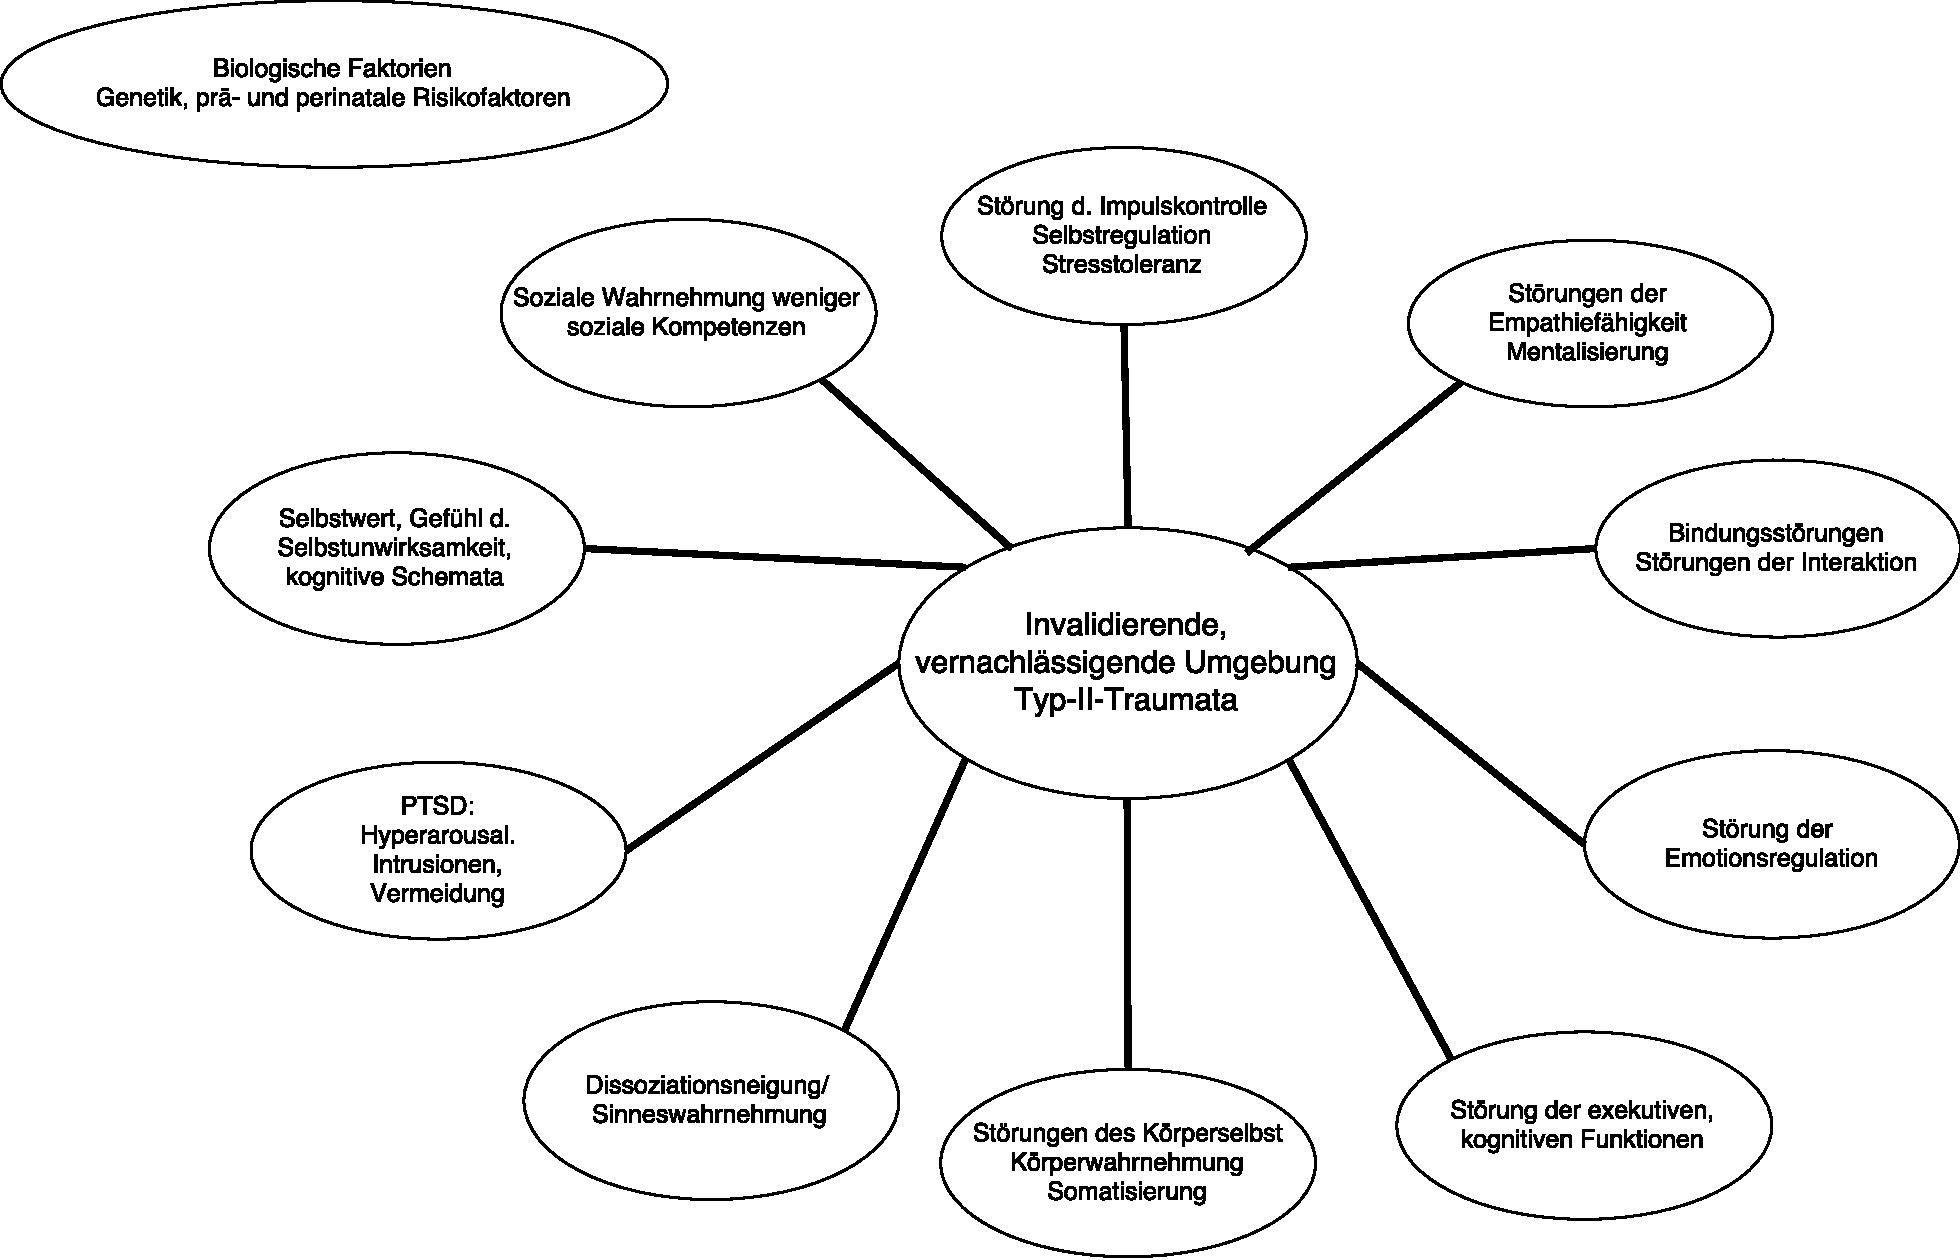
\includegraphics[scale=0.45]{abbildung4}
  \caption
      [Folgen komplexer Traumatisierungen für die Pädagogik]
      {Folgen komplexer Traumatisierungen für die Pädagogik (nach: Schmid 2013: 43)}
  \label{fig:folgen}
\end{figure}

\subsection{Entlastung der Praxis – Wiederherstellung der Handlungsfähigkeit}
Die ersten, am meisten ausgearbeiteten und praxiserprobten traumapädagogischen Konzepte kommen aus der stationären Jugendhilfe. Die PädagogInnen in der Jugendhilfe seien immer wieder mit Kinder und Jugendlichen konfrontiert, die sie an die Grenzen ihrer Handlungsmöglichkeiten brächten (vgl. Kühn 2013: 24). Traumap{\"a}dagogik sei „als Antwort auf die Erfolglosigkeit oder Nichtwirksamkeit bestimmter Konzepte in den letzten Jahren direkt aus der pädagogischen Praxis entstanden“ (Kühn 2013: 25). Die Geschichte der Heimerziehung sei „eine Geschichte von Trauma und Retraumatisierung“ (ebd.), und bis heute werde sich selten gründlich mit dem Scheitern der einzelnen Hilfsmaßnahmen auseinandergesetzt. Meistens werden die zu Betreuenden als nicht tragbar für die Einrichtung erachtet und weiterverwiesen (vgl. ebd.).

Auch Schmid (2013: 38 ff.) thematisiert die häufigen Beziehungsabbrüche den Jugendlichen (auch innerhalb der Jugendhilfe), die sich in stationären Maßnahmen befinden, was sich wiederum auf deren Bindungsfähigkeit auswirke und die aktuellen Beziehungen beeinflussen könne. Die Abbrüche und Wechsel der Institutionen entstehen laut Schmid (vgl. ebd.) oft infolge von Überforderung des sozialpädagogischen Teams mit den Symptomen des Kindes oder Jugendlichen, was zu Gefühlen der Ohnmacht und geringer Selbstwirksamkeit der Fachkräfte führt. Nicht selten wird in diesen Fällen psychotherapeutische Unterstützung für das betroffene Kind gefordert. Weiter beschreibt Schmid, wie die Erwartung an psychotherapeutische Interventionen nicht erfüllt werden kann, wenn zwischen der Pädagogik und der Psychotherapie kein gemeinsames Fallverständnis gelingt. Als nächste Maßnahme für das Kind oder den Jugendlichen (und zur Entlastung des Teams) soll nicht selten die Aufnahme in die Kinder- und Jugendpsychiatrie erfolgen. Die erforderlichen intensiven Betreuungssettings sind allerdings nicht ausreichend vorhanden, und viele Kinder und Jugendliche, die ein intensiveres Angebot benötigen, müssen abgewiesen werden. Um diesen „Kreislauf aus Ohnmacht und Ausstoßung“ (Schmid 2013: 42) zu unterbrechen, seien pädagogische Konzepte entwickelt worden, die an den Traumafolgestörungen und deren pädagogischen Folgen ansetzten. Belastete Kinder zeigen Verhaltensweisen, die ohne das Wissen um potenzielle traumabedingte Ursachen nicht adäquat beantwortet werden bzw. die Symptomatik verschärfen können (vgl. ebd.). Die MitarbeiterInnen und Teams müssen, so Schmid u. a. (2014: 185), vor Burn-out und der Möglichkeit einer sekundären Traumatisierung, die sich aus dem Arbeitskontext mit Traumatisierten ergeben, geschützt werden. Die traumapädagogischen Konzepte begründen gemäß Schmid die Notwendigkeit, Strukturen zu schaffen, die die Resilienz der MitarbeiterInnen fördern. Denn die Qualitätssicherung dient dem Wohle der PatientInnen (vgl. ebd.).

\subsection{Zur Bedeutung der Traumapädagogik im pädagogischen Alltag}
Der Bedarf an traumazentrierter Pädagogik wird aus den Möglichkeiten, die der pädagogische Alltag zur Unterstützung der Bewältigung der Traumatisierungsfolgen bietet, abgeleitet (vgl. Weiß 2016b: 20; Hantke 2015: 123 f.). Kinder und Jugendliche, die extremen Traumatisierungen ausgesetzt worden sind, zeigen oft Symptome, die ihren Alltag, auch in pädagogischen Kontexten, beeinflussen. Die pädagogischen Konzepte, die Erkenntnisse der Psychotraumatologie berücksichtigen, unterstützen die Fachkräfte, indem ihnen eine Alternative im Verstehen der Verhaltensweisen der Kinder angeboten wird sowie einige methodische Zugänge zur Verfügung gestellt werden, um mit den Symptomen des Traumas wie Übererregung, Dissoziation oder traumatische Übertragung im Alltag zu arbeiten (siehe z. B. Weiß 2016a: 290 ff.). In der Gesellschaft sowie unter den PädagogInnen wird meist die Psychotherapie als geeignete Methode zur Behandlung von Folgen der psychischen Traumata angesehen (vgl. Weiß 2003: 65). Die Auseinandersetzung mit den Traumafolgen und psychischen Störungen im Allgemeinen wird somit an den geschlossenen Raum der Therapie delegiert, so Weiß. An dieser Stelle wird gefordert, therapeutisches Wissen in die P{\"a}dagogik in einem Konzept der Zusammenarbeit von P{\"a}dagogik und Therapie zu integrieren (vgl. Weiß 2013: 20).

Mittlerweile stehen mehrere traumapsychotherapeutische Verfahren zur Verfügung, die zugleich ihre Einschränkungen aufweisen (Übersicht bei Landolt \& Hensel 2008). Unabhängig von der Therapierichtung werden drei Phasen der Traumaverarbeitung unterschieden: (1) Stabilisierung, (2) Traumabearbeitung und (3) Integration (vgl. Landolt \& Hensel 2008: 20; Huber 2003: 19). Als Standard für die psychotherapeutische Behandlung von Traumafolgen gilt, die Betroffenen nicht zu früh mit den traumatischen Erfahrungen zu konfrontieren (vgl. Purtscher-Penz 2015: 98). Zuerst soll eine stabile und tragfähige Beziehung aufgebaut werden. Kinder und Jugendliche brauchen Sicherheit, Geborgenheit und Verlässlichkeit. Erst dann können sie sich mit der traumatischen Erfahrung auseinandersetzen. Diese Auseinandersetzung ist als eine traumaspezifische psychotherapeutische Intervention durchzuführen, so Purtscher-Penz. Ziel der therapeutischen Intervention ist es, die traumabezogene Symptomatik wie Angstsymptome, einschränkendes Vermeidungsverhalten ebenso zu reduzieren wie dissoziative Zustände. In einigen Fällen kommt ergänzende psychopharmakologische Behandlung bei sehr ausgeprägter Angstsymptomatik oder Schlafstörungen hinzu (vgl. ebd.).  

Schmid u. a. (2007: 335) warnen vor unreflektierter und vordergründiger Übernahme prim{\"a}r therapeutischer Techniken in andere Settings. F{\"u}r den Erfolg einer Maßnahme sei p{\"a}dagogische Kernarbeit zur Stabilisierung entscheidender (vgl. ebd.). Komplex traumatisierte Kinder und Jugendliche brauchen neben der Psychotherapie auch eine adäquate Pädagogik im Alltag, die Sicherheit und Kontinuität gewährleistet (vgl. Purtscher-Penz 2015: 99; Hensel 2014: 34). Die aus der Traumatisierung resultierenden Beeinträchtigungen, besonders bei komplex Traumatisierten, wirken im Alltag und bedürfen entsprechender pädagogischer Interventionen, so Schmid (2013: 47, siehe Abbildung \ref{fig:ansatzpunkte}). Diese können auch im pädagogischen Alltag verfolgt werden. Dazu gehört, einen sicheren Ort zu vermitteln, der vor Retraumatisierungen\footnote{Ein Zustand der Betroffenen Person, in der eine erneute Erinnerung an das traumatische Erlebnis direkt zu einer erh{\"o}hten Symptombelastung f{\"u}hrt (vgl. Maercker 2009: 16).} schützt und das Kind oder den Jugendlichen stabilisiert; „korrigierende Beziehungserfarungen“ durch motivierte und stabile Erwachsene anzubieten und die Emotionsregulation durch das Erlernen spezifischer Fertigkeiten zu verbessern. Die Verbesserung der Selbst-, Fremd- und Körperwahrnehmung kann die Dissoziationsneigung reduzieren. Ressourcenorientierung, Partizipation und Transparenz im Alltag sind aufgrund der vielfachen Erfahrungen des Kontrollverlustes und zur Überwindung der „Selbstunwirksamkeitserwartung [sic]“ wichtig (vgl. Schmid 2013: 47).

\begin{figure}[h]
  \centering
  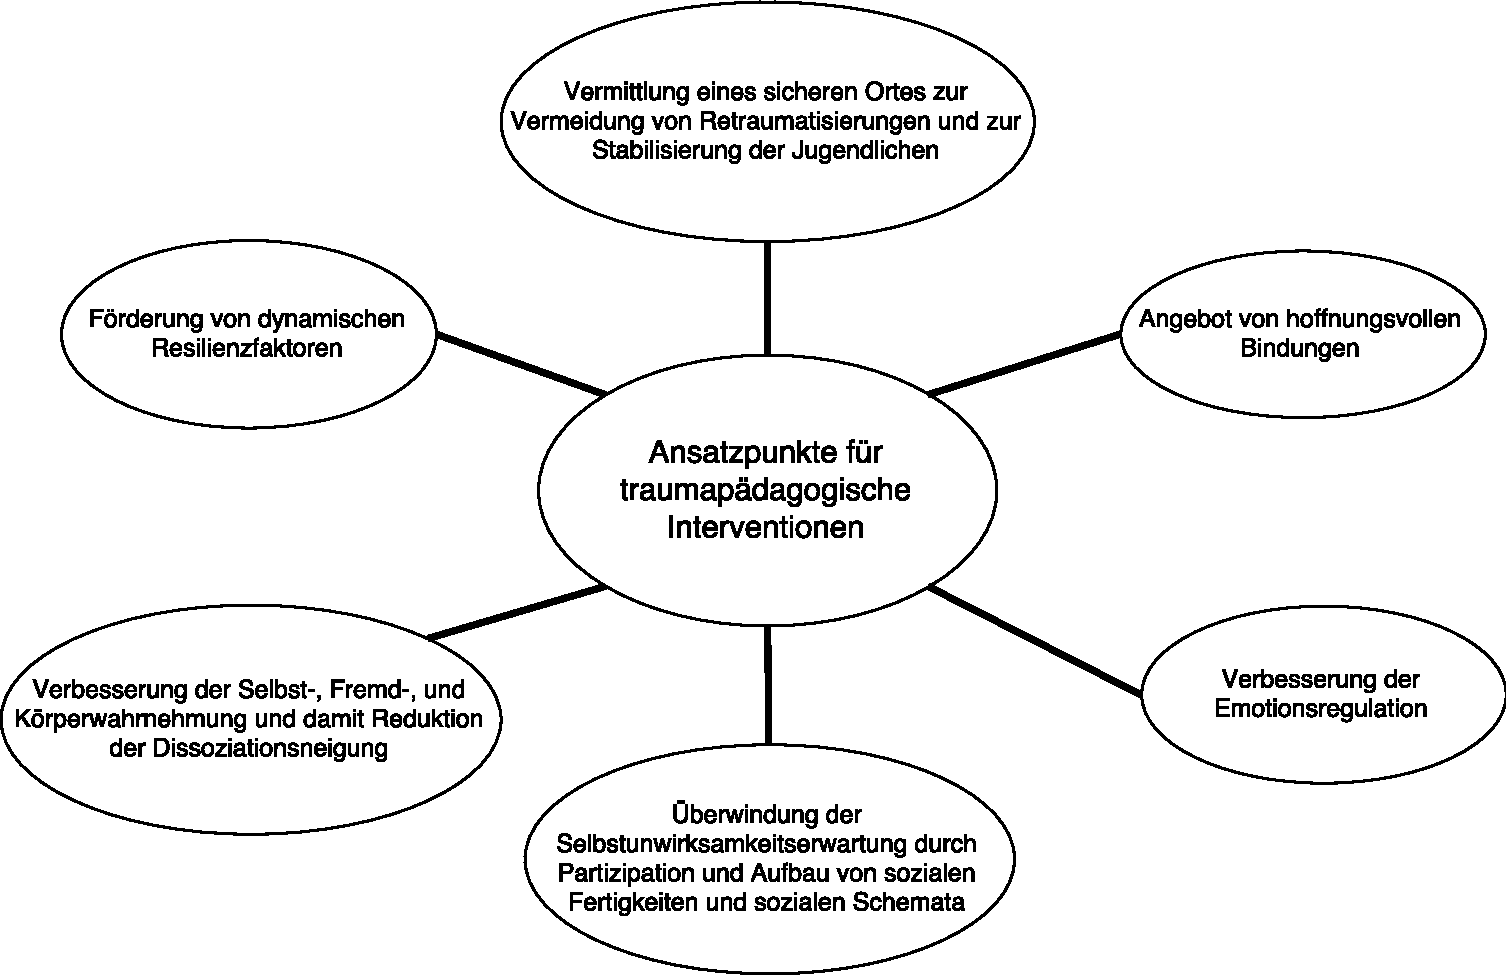
\includegraphics[scale=0.5]{abbildung5}
  \caption
      [Ansatzpunkte für traumapädagogische Interventionen]
      {Ansatzpunkte für traumapädagogische Interventionen (nach Schmid 2013: 47)}
  \label{fig:ansatzpunkte}
\end{figure}

Weiß (2013: 18 ff.) vertritt den Standpunkt, dass die Verwendung von Erkenntnissen der Traumatheorie und Traumaforschung nicht therapeutischen SpezialistInnen und WissenschaftlerInnen vorbehalten werden sollte. Vielmehr sei es wichtig, diese Erkenntnisse im Interesse der betroffenen M{\"a}dchen und Jungen und der sie begleitenden P{\"a}dagogInnen auf ihre Anwendbarkeit im pädagogischen Kontext zu {\"u}berpr{\"u}fen, da „die Unterst{\"u}tzung traumatisierter M{\"a}dchen und Jungen außerhalb des individualisierten Rahmens von Therapie auch in der P{\"a}dagogik sehr wirksam sein kann“ (Weiß 2013: 21 f.). Die therapeutische Hilfe orientiere sich idealerweise in erster Linie an dem Kind, seinem Wunsch, Alter, seiner Lebensgeschichte, dem aktuellen Wohlbefinden und seiner Stabilität (vgl. Weiß 2013: 180). Ziele der Therapie seien: korrigierende und wiedergutmachende Erfahrungen sowie Unterstützung bei der Entwicklung der Ich-Kräfte. Die Therapieziele seien auch gekoppelt an die Reaktionen der Bezugspersonen und könnten unter Umständen die Kinder und Jugendlichen in erneute Konfliktsituationen bringen (vgl. ebd.: 182). „Eine therapeutische Unterstützung bei der Verarbeitung traumatischer Erfahrungen kann nur hilfreich sein, wenn sie sorgfältig als Teil im gesamten Hilfeprozess eingebettet ist“ (ebd.). Kühn (2014: 21 f.) betont die Überschätzung der therapeutischen Möglichkeiten durch die pädagogischen Fachkräfte, was wiederum zur Unterschätzung und Entwertung der eigenen Fachkompetenz führe (ebd.). Unumstritten bleibt, dass im Rahmen der Traumap{\"a}dagogik keine Traumaexposition (Traumakonfrontation) stattfinden soll. Eine deutliche Abgrenzung zur psychotherapeutischen Intervention sei wichtig (vgl. Schmid u. a. 2007: 335).

Zusammenfassend lassen sich auf der Suche nach der Begründung für die „neue Fachdisziplin“ Traumapädagogik unter anderen vier Argumente identifizieren:

\begin{enumerate}
\item Die Anzahl der durch traumatische Erfahrungen belasteten Kinder und Jugendlichen in den pädagogischen Handlungsfeldern sei hoch.  
\item Diese Kinder und Jugendliche hätten traumabedingt besondere Bedarfe, die besonderer (trauma-)pädagogischer Maßnahmen bedürften.  
\item Die pädagogischen Fachkräfte seien ohne entsprechender Unterstützung und aufgrund der Herausforderungen, die die Traumatisierung mit sich bringe, besonderen Belastungen ausgesetzt und stießen auf Grenzen ihrer Handlungsmöglichkeiten (bis hin zur sekundären Traumatisierung der Fachkräfte).  
\item Dabei biete der pädagogische Alltag viele Möglichkeiten, die betroffene Kinder und Jugendliche in ihrer Traumabearbeitung zu unterstützen. Im Mittelpunkt dieser Überlegungen stünden vorrangig Fachkräfte und Kinder und Jugendliche, die in den stationären und teilstation{\"a}ren Einrichtungen der Jugendhilfe betreut und versorgt würden.
\end{enumerate}
